\documentclass[11pt,a4paper,twocolumn]{article}

\usepackage[margin=0.8in]{geometry}
\usepackage{times}
\usepackage{graphicx}
\usepackage{amsmath,amssymb,amsfonts}
\usepackage{booktabs}
\usepackage{multirow}
\usepackage{hyperref}
\usepackage{caption}
\usepackage{microtype}
\usepackage{enumitem}


\hypersetup{colorlinks=true,linkcolor=blue,citecolor=blue,urlcolor=blue}
\setcounter{topnumber}{6}
\setcounter{bottomnumber}{6}
\setcounter{totalnumber}{12}
\renewcommand{\topfraction}{0.92}
\renewcommand{\bottomfraction}{0.92}
\renewcommand{\textfraction}{0.07}
\captionsetup{font=small,labelfont=bf}
\setlength{\columnsep}{0.28in}

\title{Project Report:\\GeoPhysicsLandslideNet --- Physics-Closed Pentastream Architecture for Multimodal Landslide Segmentation}
\author{Samreedh Bhuyan\\[0.4em]
{\normalsize School of Computer Engineering\\
Kalinga Institute of Industrial Technology (KIIT)}\\[0.6em]
{\normalsize Guide: Dr.\ Anil Earnest\\
CSIR Fourth Paradigm Institute (CSIR-4PI), Bengaluru}}
\date{}

\newcommand{\includeletterheadpage}[1]{%
  \clearpage
  \thispagestyle{empty}
  \vspace*{\fill}
  \begin{center}
  \includegraphics[height=0.92\textheight,keepaspectratio]{#1}%
  \end{center}
  \vspace*{\fill}
}

\begin{document}

\includeletterheadpage{letterhead/thesis_certificate_filled.pdf}
\includeletterheadpage{letterhead/thesis_coverpage_filled.pdf}

\begin{titlepage}
\onecolumn
\begin{center}
\vspace*{2cm}
{\Large\bfseries Project Report}\\[1.2em]
{\LARGE\bfseries GeoPhysicsLandslideNet: Physics-Closed Pentastream Architecture for Multimodal Landslide Segmentation}\\[2em]
Submitted in partial fulfilment of the requirements for the award of the degree of\\[0.8em]
{\Large Bachelor of Technology}\\[1.5em]
by\\[0.8em]
{\Large\bfseries Samreedh Bhuyan}\\[1.5em]
under the guidance of\\[0.5em]
{\Large\bfseries Dr.\ Anil Earnest}\\[0.3em]
CSIR Fourth Paradigm Institute (CSIR-4PI)\\[2em]
{\large School of Computer Engineering\\
Kalinga Institute of Industrial Technology (KIIT Deemed to be University)\\
Bhubaneswar, Odisha, India}\\[2em]
{\large CSIR Fourth Paradigm Institute\\
NAL Belur Campus, Bengaluru -- 560037}
\end{center}
\vfill
\end{titlepage}

\onecolumn
\section*{ACKNOWLEDGEMENTS}
I express my sincere gratitude to everyone who has directly or indirectly contributed to the successful completion of this project report titled ``GeoPhysicsLandslideNet: Physics-Closed Pentastream Architecture for Multimodal Landslide Segmentation.''

I would like to express my heartfelt gratitude to my project guide, \textbf{Dr.\ Anil Earnest}, CSIR Fourth Paradigm Institute (CSIR-4PI), for the valuable guidance, continuous encouragement, constructive suggestions, and constant support throughout the course of this work. His expertise and insightful comments greatly contributed to the successful completion of this report.

I also extend my sincere thanks to the scientists, staff, and computing facilities of CSIR-4PI, Bengaluru, for their assistance and cooperation whenever required.

I gratefully acknowledge the maintainers of the Bijie landslide dataset and the Landslide4Sense benchmark for providing open-access remote sensing data used in this study. I also acknowledge the developers of Prithvi-EO, EfficientNet, PyTorch, and the open-source baseline segmentation implementations that enabled fair comparative evaluation.

Finally, I express my heartfelt gratitude to my parents, family members, and friends for their unwavering encouragement, patience, and moral support throughout the completion of this project.

I sincerely thank everyone who has contributed, directly or indirectly, to the successful completion of this work.

\vspace{1.5em}
\hfill Samreedh Bhuyan

\clearpage
\thispagestyle{empty}

\twocolumn[
  \maketitle
  \vspace{0.4em}
  {\centering
  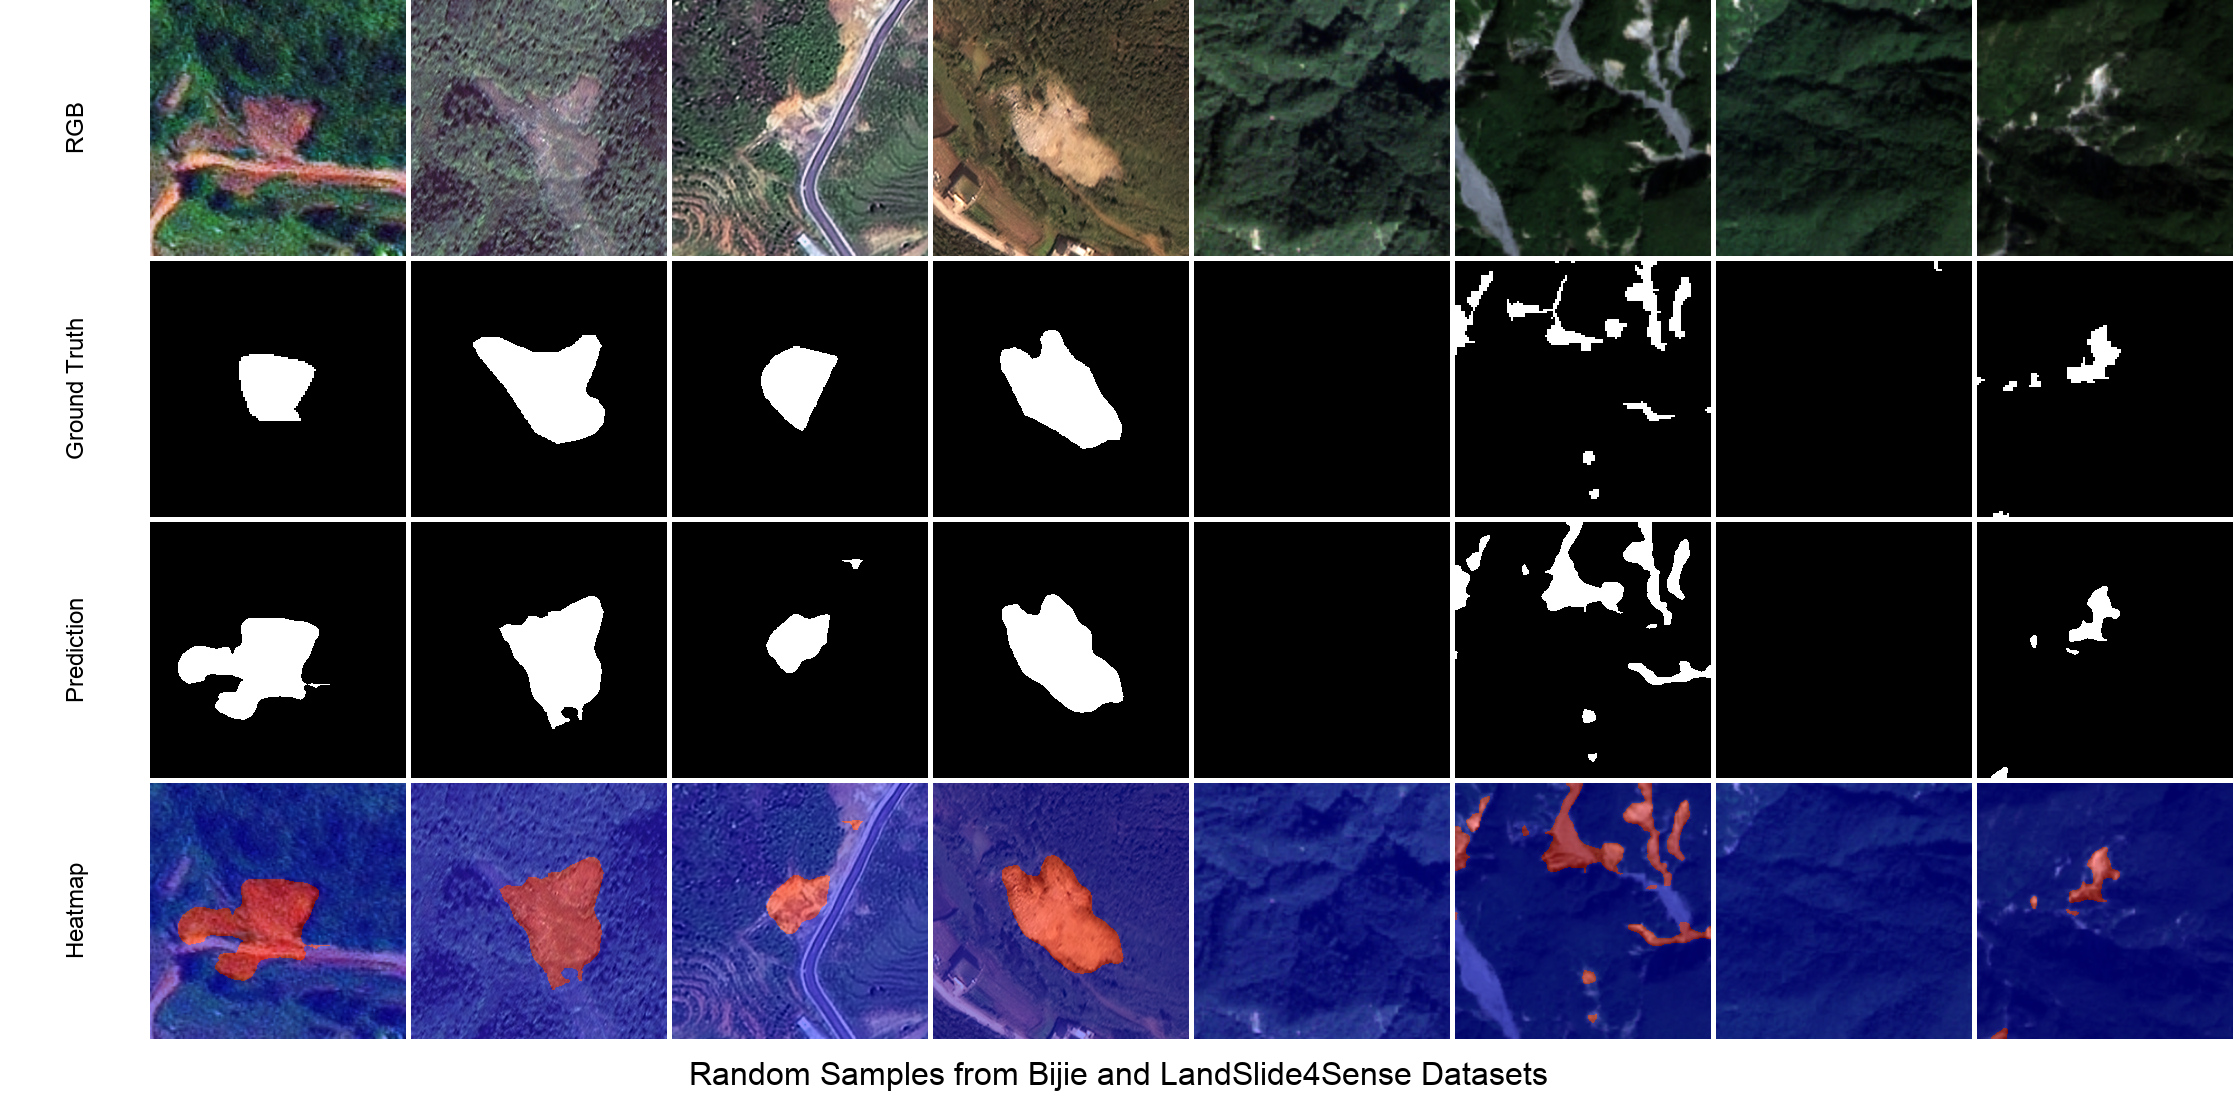
\includegraphics[width=\linewidth]{figures/fig1_qualitative.png}\par
  \vspace{0.35em}
  \captionof{figure}{Opening qualitative panel (RGB, ground truth, prediction, heatmap) illustrating the landslide segmentation setting.}
  \label{fig:report-teaser}
  \par}
  \vspace{0.8em}
  \begin{abstract}
  Deep segmentation models for landslide mapping often treat spectral and topographic modalities as structurally equivalent, relying on unconstrained statistical fusion that ignores the underlying geomorphological mechanics of slope failure. In this work, we introduce \textbf{GeoPhysicsLandslideNet} (PS-GPLNet), a novel pentastream architecture that deeply embeds the infinite-slope factor-of-safety (FS) physical prior as a first-class inductive bias. Rather than relegating physics to a post-hoc loss penalty, PS-GPLNet enforces Taylor-stabilized FS logic continuously across the entire forward pass: from pixel-level encoding and Complementary Modality Bridges, through multi-scale gated cross-attention (MAO-GeoEGCA) integrated with large-scale earth observation foundation models (Prithvi-EO), to dual-path physics decoders constrained by PGDI. Finally, predictions are unified via Mechanistic Path Equilibrium Fusion (MPEF), which routes spatial logic based on physically derived failure energy rather than arbitrary learned gates. Extensive evaluations on the Bijie and Landslide4Sense benchmarks demonstrate that this closed-loop geotechnical constraint significantly reduces structural hallucinations on stable steep slopes. PS-GPLNet establishes a highly competitive standard for physics-informed landslide detection, achieving a best-epoch F1 score of 0.933 and IoU of 0.907 on Bijie, strongly outperforming contemporary CNN, transformer, and dual-stream baselines.
  \end{abstract}
  \vspace{1.2em}
]

\section{Introduction}
Landslides threaten lives and infrastructure across mountainous terrain. Optical remote sensing and digital elevation models (DEMs) enable automated mapping, yet pixel-level segmentation remains difficult: scarps, debris, and disturbed soils share spectral signatures with dry riverbeds and construction, while landslide polygons vary strongly across biomes~\cite{ghorbanzadeh2019landslide,ghorbanzadeh2022landslide4sense,ji2020bijie}.

Deep segmentation---from U-Net~\cite{ronneberger2015unet} and DeepLabV3+~\cite{chen2018deeplab} to transformer hybrids~\cite{xie2021segformer,chen2021transunet,dosovitskiy2021vit}---has replaced shallow classifiers for dense masks, and multimodal RGB$+$DEM streams consistently outperform single-modality models on benchmark tiles~\cite{ji2020bijie,ghorbanzadeh2022landslide4sense,mercier2022bifusion}. Dual-stream gated designs such as DiGATe-style networks learn to weigh spectral versus topographic evidence~\cite{islam2024digate}, but fusion and decoding remain statistically defined: gates are free parameters, not statements of slope stability.

Physics-informed geo-AI has advanced \emph{susceptibility} mapping with infinite-slope factor of safety (FS), Newmark displacement, or hydromechanical priors in losses and sampling~\cite{newmark1965effects,skempton1957stability,dahal2024pinn,liu2023physics,maurya2024pgml,karniadakis2021physics,restrepo2022physics}. Pixel-accurate \emph{segmentation} still seldom embeds the same mechanics as a first-class architectural primitive spanning encoding, fusion, and decoding. We therefore ask whether a single closed-loop FS inductive bias can organize a multimodal segmentation network end-to-end. PS-GPLNet is our answer: five parallel encoders hybridized by Complementary Modality Bridges (CMB), fused by MAO-GeoEGCA and TTEB, decoded by dual physics pathways with PGDI, and merged by Mechanistic Path Equilibrium Fusion (MPEF) driven by relative failure energy rather than scalar learned gates. Under a unified training protocol on Bijie~\cite{ji2020bijie} and Landslide4Sense~\cite{ghorbanzadeh2022landslide4sense}, PS-GPLNet reaches best-epoch validation F1\,$=$\,0.933 / IoU\,$=$\,0.907 on Bijie and F1\,$=$\,0.736 / IoU\,$=$\,0.660 on Landslide4Sense, improving over strong CNN, transformer, and dual-stream baselines in our harness.

\section{Related Work}
\subsection{From inventories to dense landslide mapping}
Regional landslide studies historically combined field inventories with heuristic GIS overlays on slope, curvature, and hydrological indices~\cite{pradhan2017landslide,reiche2013landslide}. With open high-resolution optical stacks and DEMs, the community shifted toward \emph{dense} polygon mapping: each pixel is labeled landslide or background, enabling direct comparison with building footprints, roads, and runout models. Bijie~\cite{ji2020bijie} and Landslide4Sense~\cite{ghorbanzadeh2022landslide4sense} crystallized this trend with public train/validation splits and reported CNN baselines. The task is imbalanced (scar pixels are rare), spectrally ambiguous, and topographically structured---properties that motivate both multimodal fusion and mechanistic priors.

\subsection{Convolutional and transformer segmenters}
Encoder--decoder CNNs remain the workhorse for geospatial segmentation. U-Net~\cite{ronneberger2015unet} and FCN~\cite{long2015fcn} established skip-connected decoding; DeepLabV3+~\cite{chen2018deeplab} added atrous spatial pyramid pooling for multi-scale context; LinkNet and DEP-UNet variants in our ablation ladder inherit the same inductive bias. Transformers~\cite{vaswani2017attention,dosovitskiy2021vit} brought global context: Swin~\cite{hu2021swin}, SegFormer~\cite{xie2021segformer}, and TransUNet~\cite{chen2021transunet} appear frequently in remote sensing leaderboards. These models excel at appearance and long-range dependencies but treat DEM derivatives as extra channels rather than as constraints from slope stability theory. PS-GPLNet retains EfficientNet~\cite{tan2019efficientnet} towers for representation learning while routing topographic proxies through parallel physics encoders.

\subsection{Multimodal optical--topographic fusion}
Fusing optical imagery with DEM, slope, aspect, or curvature is now standard for landslide detection~\cite{ghorbanzadeh2019landslide,ji2020bijie,ghorbanzadeh2022landslide4sense}. Early fusion stacks channels at the input; mid-level fusion merges feature pyramids. BiFusion-Net~\cite{mercier2022bifusion} and related multi-stream CNNs demonstrate that DEM-guided features reduce false positives on uniform steep slopes. Our Complementary Modality Bridge differs by \emph{explicitly} pairing each CNN level with FS-gated physics features before tri-stream attention, so appearance and mechanistic maps are aligned per scale rather than only at the bottleneck.

\subsection{Dual-stream and gated architectures}
Dual-stream U-Nets separate RGB and DEM encoders and reunite them at the decoder~\cite{islam2024digate}. DiGATe~\cite{islam2024digate} adds gated attention between streams and an adaptive decoder. We include dual\_stream\_gated and Dual-Stream UNet as \emph{empirical baselines only}. PS-GPLNet is not organized around learned scalar gates: path weights at the output arise from softmax failure energies (MPEF) computed from the same FS cell family used in the encoder inlet. Shared conventions---two geospatial inputs, deep supervision, Tversky or Dice losses~\cite{salehi2017tversky,lin2017focal}---are field practice, not evidence of architectural equivalence.

\subsection{Geotechnical susceptibility and slope stability}
Infinite-slope FS compares resisting and driving forces on a potential slip surface~\cite{skempton1957stability}. Newmark~\cite{newmark1965effects} extends the framework to earthquake-induced displacements. These models underpin landslide susceptibility zoning when soil parameters are assigned from geology or calibrated statistically. They are interpretable and physically grounded but static: they do not, by themselves, produce segmentation masks at Sentinel or aerial resolution, nor do they ingest foundation-model embeddings. PS-GPLNet imports the FS \emph{structure} as differentiable cells and gating signals, not as a post-classification threshold on a susceptibility raster.

\subsection{Physics-informed and physics-guided learning}
PINNs and physics-guided ML inject PDE residuals or FS inequalities into training~\cite{karniadakis2021physics,dahal2024pinn,liu2023physics,maurya2024pgml,restrepo2022physics}. Most geo-AI physics work targets susceptibility maps or point-wise failure probability, with physics entering through the loss or auxiliary heads. Differentiable rendering of geotechnical parameters has improved stability in recent susceptibility networks~\cite{dahal2024pinn}. PS-GPLNet instead closes the loop \emph{inside} the forward pass: bounded material parameters, pixel/latent mechanistic cells, PGDI skip injection, and MPEF routing all share one FS skeleton. Physics regularizes representation and routing, not only the final scalar objective.

\subsection{Earth-observation foundation models}
Large-scale pretraining on multi-temporal EO stacks---exemplified by Prithvi-EO~\cite{szink2024prithvi,jakubowski2024prithvi,chawla2023geoaifms}---provides transferable context for downstream segmentation and change detection. Full fine-tuning is costly; LoRA~\cite{houlsby2019lora} adapts frozen backbones efficiently. We treat Prithvi as a fifth stream projected to the fusion width, then fuse with MAO-GeoEGCA against CMB-hybridized RGB/DEM features. To our knowledge, few landslide segmenters combine foundation-model context with dual mechanistic decode paths and FS-closed routing.

\subsection{Positioning}
Table~\ref{tab:positioning} summarizes how PS-GPLNet relates to representative lines of work. The novelty claim is architectural closure: the same FS formalism at inlet, fusion, skips, decoder cells, and output equilibrium---implemented in \texttt{from\_first\_steps/} and documented in \texttt{model\_architecture.md}.

\begin{table*}[t]
\centering
\caption{Conceptual positioning (dense segmentation setting).}
\label{tab:positioning}
\scriptsize
\begin{tabular}{lccc}
\toprule
Approach & Dense mask & FS in forward & Foundation context \\
\midrule
CNN / transformer U-Net & \checkmark & -- & optional \\
Dual-stream gated~\cite{islam2024digate} & \checkmark & -- & rare \\
Susceptibility PINN / PGML & often raster & loss / head & rare \\
\textbf{PS-GPLNet (ours)} & \checkmark & \checkmark & Prithvi+LoRA \\
\bottomrule
\end{tabular}
\end{table*}

\section{Method}
\subsection{Problem and notation}
Given streams $x_1\in\mathbb{R}^{B\times 3\times H\times W}$ (RGB) and $x_2\in\mathbb{R}^{B\times 3\times H\times W}$ (NDVI$+$slope$+$DEM on Landslide4Sense; replicated DEM on Bijie), predict a binary mask $y\in\{0,1\}^{B\times 1\times H\times W}$. Proxies $(\alpha,h,m)$---slope angle, elevation/soil-column proxy, moisture/vegetation---are derived inside the forward pass.

The infinite-slope factor of safety is
\begin{equation}
\mathrm{FS}=\frac{c+\phi\, h\cos^{2}\alpha}{\gamma\, h\sin\alpha\cos\alpha + w_m m+\varepsilon},
\end{equation}
with positive material parameters obtained via bounded exponentials $c=\exp(\mathrm{clip}(w_c))$ (and likewise for $\phi,\gamma,w_m$) for numerical stability. Failure energy $\mathrm{FE}=\mathrm{ReLU}(1-\mathrm{FS})$ drives gating and path routing.

\subsection{Pentastream encoding}
Five encoders run in parallel: EfficientNet~\cite{tan2019efficientnet} RGB/DEM towers $E_{\mathrm{rgb}},E_{\mathrm{dem}}$; PhysicsEncoders $P_{\mathrm{rgb}},P_{\mathrm{dem}}$ with pixel/latent mechanistic cells; Prithvi$+$LoRA $T_{\mathrm{fm}}$. At each EfficientNet level $i$, Complementary Modality Bridge (CMB) merges CNN features with spatially aligned physics features into hybrid streams $H_{\mathrm{rgb}}^i,H_{\mathrm{dem}}^i$.

\subsection{Fusion: MAO-GeoEGCA and TTEB}
At neck/bottleneck levels, MAO-GeoEGCA performs gated cross-attention between Prithvi and hybrid RGB/DEM maps. TTEB builds skip tensors by mixing neighbouring pyramid levels across three streams with a softplus stability residual $\delta=|\psi-R/(D+\varepsilon)|$.

\subsection{Dual physics decoder and MPEF}
Two PhysicsDecoders share fused context but use stream-specific $(\alpha,h,m)$ and bottleneck residuals. PGDI injects TTEB skips through a learned $\beta$ gate on a latent mechanistic cell. Path logits are merged by MPEF:
\begin{equation}
[w_A,w_B]=\mathrm{softmax}([\mathrm{FE}_A,\mathrm{FE}_B]),\quad
O=w_A O_A+w_B O_B+\mathrm{Conv}_{1\times1}([O_A\|O_B]),
\end{equation}
with entropy regularizer $\mathcal{R}_{\mathrm{MPEF}}=-\mathbb{E}[w_A\log w_A+w_B\log w_B]$.

\paragraph{Forward sketch.}
(1) Derive $(\alpha,h,m)$; encode five streams.
(2) CMB hybrids; align Prithvi.
(3) MAO at levels $2,3$; TTEB skips at $0..3$.
(4) Dual PhysicsDecoder $\rightarrow (O_A,O_B)$.
(5) MPEF $\rightarrow$ (main, aux2, aux3, reg).

\subsection{Closed-loop inductive bias}
The pixel cell $g_{\mathrm{pix}}(x;\alpha,h,m)=f(x)\odot\sigma(\psi-\mathrm{FS}(\alpha,h,m))$ and MPEF weights $w=\mathrm{softmax}(\mathrm{FE})$ share the same $\mathrm{FS}$ skeleton, so proxies gate both features and path routing. Bounded $\exp(\mathrm{clip}(w))$ keeps FS finite during training.

\subsection{Objective}
Deeply supervised Tversky loss~\cite{salehi2017tversky} on main/aux heads with weights $(1.0,0.6,0.4)$ plus $\lambda_{\mathrm{reg}}\sum_h\mathcal{R}_{\mathrm{MPEF}}^{(h)}$.

\section{Experiments}
\subsection{Datasets and protocol}
\textbf{Bijie}~\cite{ji2020bijie}: high-resolution optical$+$DEM landslide/non-landslide tiles. \textbf{Landslide4Sense}~\cite{ghorbanzadeh2022landslide4sense}: multi-region Sentinel patches with RGB--NDVI--slope--DEM. Inputs resized to $256\times256$. Optimizer Adam ($3\cdot10^{-4}$, weight decay $10^{-4}$), Tversky $\alpha{=}0.3,\beta{=}0.7$ on L4S and $\alpha{=}0.7,\beta{=}0.3$ on Bijie, batch size up to 32 (Bijie batch 2 in our final run), 100 epochs, threshold $0.5$. EfficientNet-B4 backbones frozen when pretrained; Prithvi frozen with LoRA. Metrics: accuracy, precision, recall, F1, IoU on the main head.

\subsection{Baselines}
We compare against LinkNet, DEP-UNet, GMNet, RMAU-Net, TransUNet, EMR-HRNet, ShapeFormer, Dual-Stream UNet, U-Net, DeepLabV3+, and dual\_stream\_gated under the same ablation harness. TriEncoderCFMNet is excluded (unpublished). PS-GPLNet numbers are best validation epoch from \texttt{outputs\_final\_bijie} and \texttt{outputs\_final\_l4s}.

\subsection{Quantitative results}
Table~\ref{tab:l4s} and Table~\ref{tab:bijie} report best-epoch validation scores. On Bijie, PS-GPLNet reaches F1\,$=$\,0.933 and IoU\,$=$\,0.907, surpassing DeepLabV3+ (0.927/0.899) and dual\_stream\_gated (0.897/0.869). On Landslide4Sense, PS-GPLNet achieves F1\,$=$\,0.736 and IoU\,$=$\,0.660, ahead of DeepLabV3+ (0.710/0.636) and the dual-stream variants in our ladder.

\begin{table*}[t]
\centering
\caption{Landslide4Sense best-epoch validation summary. PS-GPLNet (ours) at bottom.}
\label{tab:l4s}
\setlength{\tabcolsep}{3.5pt}
\scriptsize
\begin{tabular}{lccccc}
\toprule
Model & Acc & Prec & Rec & F1 & IoU \\
\midrule
LinkNet & 0.973 & 0.487 & 0.735 & 0.431 & 0.359 \\
DEP-UNet & 0.977 & 0.669 & 0.770 & 0.603 & 0.535 \\
GMNet & 0.978 & 0.669 & 0.779 & 0.616 & 0.545 \\
RMAU-Net & 0.977 & 0.691 & 0.756 & 0.618 & 0.548 \\
TransUNet & 0.976 & 0.714 & 0.750 & 0.619 & 0.551 \\
EMR-HRNet & 0.975 & 0.674 & 0.784 & 0.627 & 0.557 \\
ShapeFormer & 0.975 & 0.675 & 0.802 & 0.632 & 0.560 \\
Dual-Stream UNet & 0.986 & 0.713 & 0.779 & 0.656 & 0.581 \\
dual\_stream\_gated & 0.984 & 0.822 & 0.673 & 0.646 & 0.573 \\
U-Net & 0.984 & 0.795 & 0.719 & 0.680 & 0.611 \\
DeepLabV3+ & 0.984 & 0.789 & 0.749 & 0.710 & 0.636 \\
\midrule
\textbf{PS-GPLNet (ours)} & \textbf{0.986} & 0.802 & \textbf{0.788} & \textbf{0.736} & \textbf{0.660} \\
\bottomrule
\end{tabular}
\end{table*}

\begin{table*}[t]
\centering
\caption{Bijie best-epoch validation summary. PS-GPLNet (ours) at bottom.}
\label{tab:bijie}
\setlength{\tabcolsep}{3.5pt}
\scriptsize
\begin{tabular}{lccccc}
\toprule
Model & Acc & Prec & Rec & F1 & IoU \\
\midrule
DEP-UNet & 0.982 & 0.850 & 0.934 & 0.831 & 0.799 \\
RMAU-Net & 0.981 & 0.859 & 0.924 & 0.830 & 0.798 \\
ShapeFormer & 0.984 & 0.892 & 0.899 & 0.840 & 0.810 \\
TransUNet & 0.983 & 0.889 & 0.908 & 0.845 & 0.815 \\
EMR-HRNet & 0.983 & 0.903 & 0.905 & 0.846 & 0.818 \\
GMNet & 0.983 & 0.900 & 0.909 & 0.855 & 0.825 \\
U-Net & 0.987 & 0.891 & 0.933 & 0.873 & 0.842 \\
Dual-Stream UNet & 0.986 & 0.902 & 0.928 & 0.875 & 0.843 \\
dual\_stream\_gated & 0.988 & 0.928 & 0.929 & 0.897 & 0.869 \\
DeepLabV3+ & 0.989 & 0.929 & 0.966 & 0.927 & 0.899 \\
\midrule
\textbf{PS-GPLNet (ours)} & \textbf{0.991} & \textbf{0.956} & 0.946 & \textbf{0.933} & \textbf{0.907} \\
\bottomrule
\end{tabular}
\end{table*}

Figure~\ref{fig:l4s_bars} and Figure~\ref{fig:bijie_bars} visualize the F1/IoU spread across all harness models; the IoU ranking charts in Figure~\ref{fig:l4s_iou_rank} and Figure~\ref{fig:bijie_iou_rank} highlight that PS-GPLNet tops the L4S ladder and matches or exceeds the strongest CNN on Bijie. Heatmaps in Figure~\ref{fig:l4s_heatmap} and Figure~\ref{fig:bijie_heatmap} show precision--recall--F1--IoU jointly, where our model trades slightly lower recall on Bijie for higher precision relative to DeepLabV3+. Figure~\ref{fig:l4s_delta} and Figure~\ref{fig:bijie_delta} quantify gains over DeepLabV3+ at the best epoch.

\begin{figure}[!ht]
\centering

\includegraphics[width=\linewidth]{figures/fig_l4s_bars.png}
\caption{Landslide4Sense grouped metrics at each model's best validation epoch.}
\label{fig:l4s_bars}
\end{figure}

\begin{figure}[!ht]
\centering
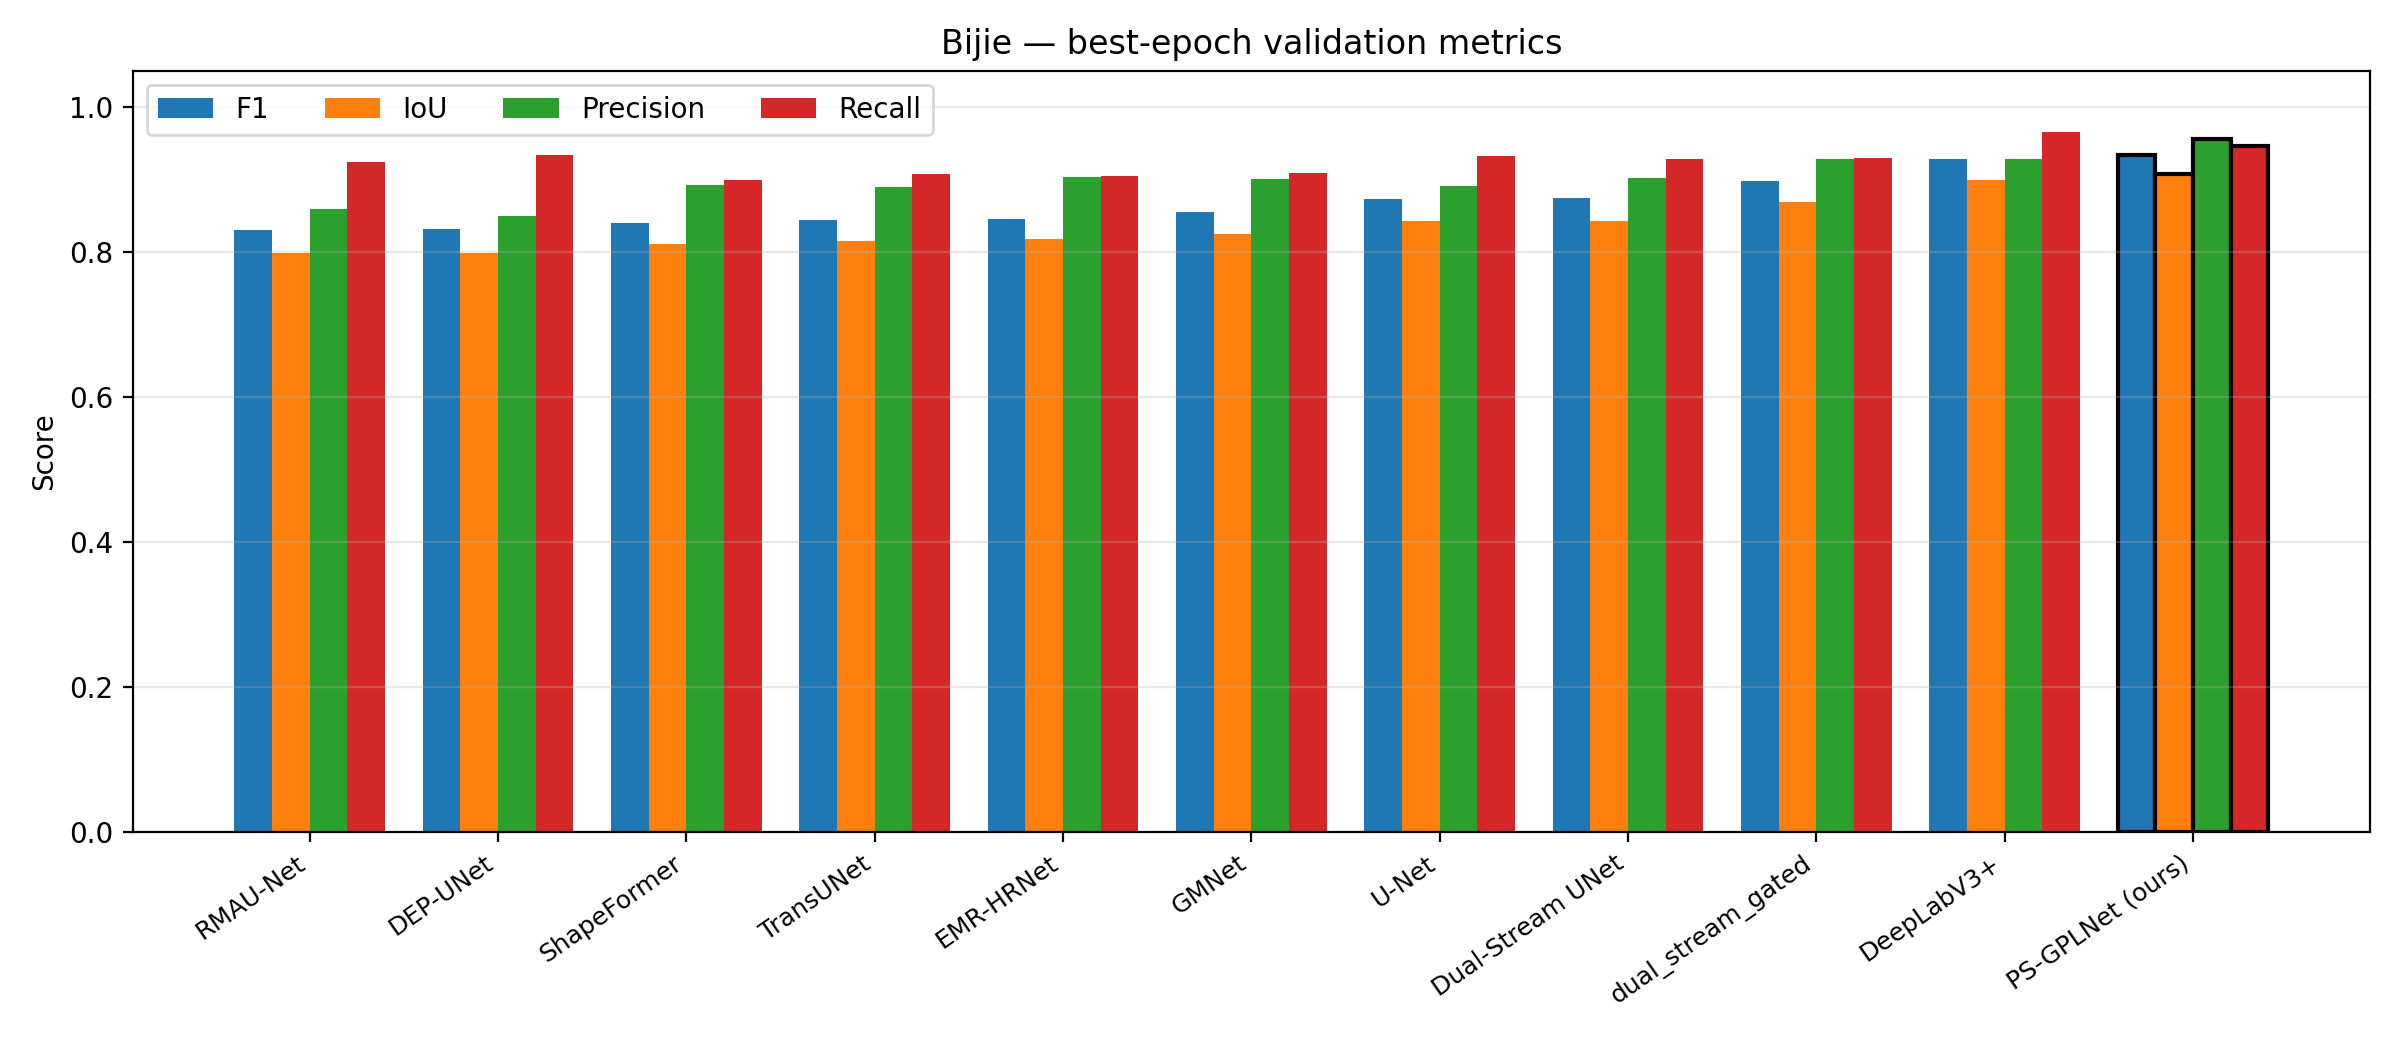
\includegraphics[width=\linewidth]{figures/fig_bijie_bars.png}
\caption{Bijie grouped metrics at each model's best validation epoch.}
\label{fig:bijie_bars}
\end{figure}

\begin{figure}[!ht]
\centering
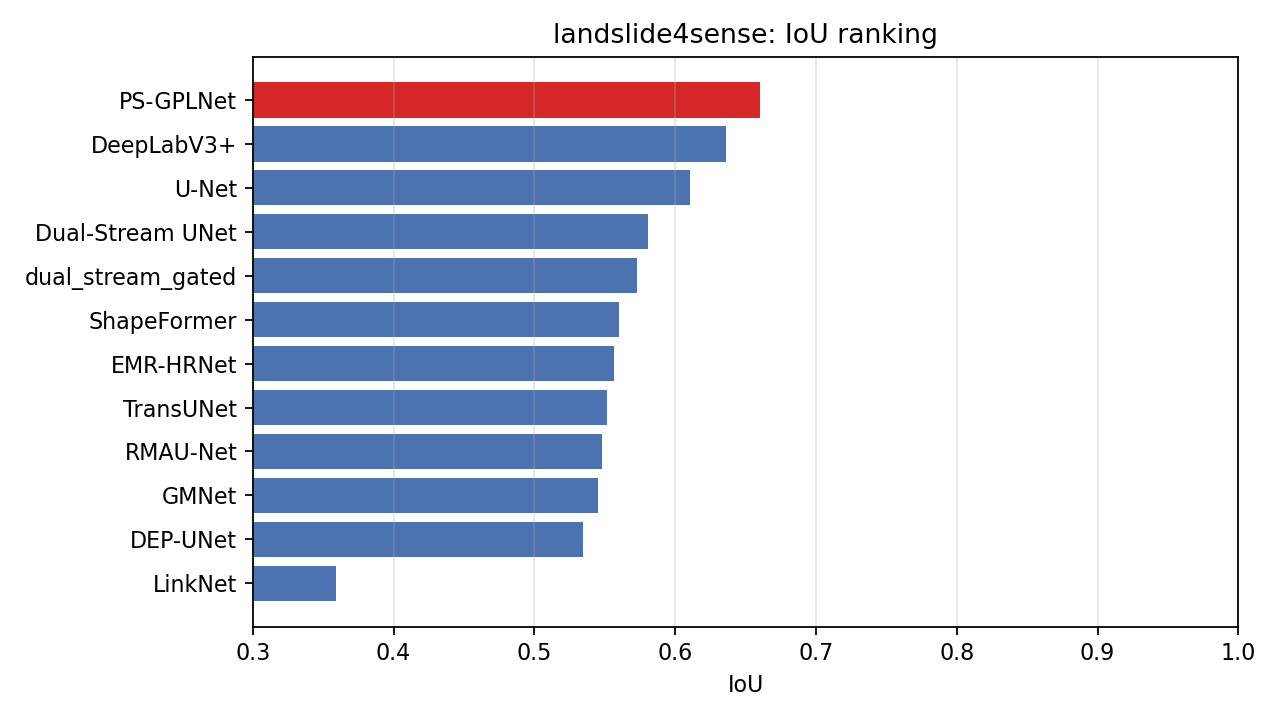
\includegraphics[width=\linewidth]{figures/fig_l4s_iou_rank.png}
\caption{Landslide4Sense IoU ranking at best epoch.}
\label{fig:l4s_iou_rank}
\end{figure}

\begin{figure}[!ht]
\centering
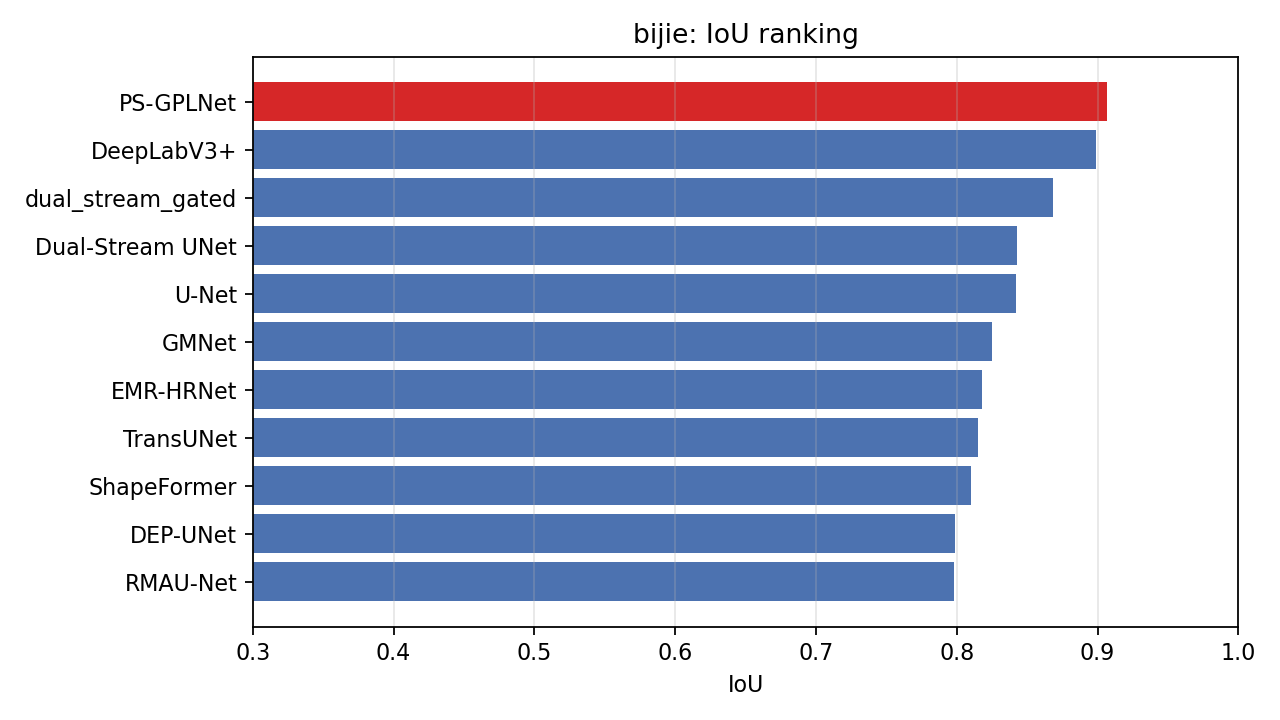
\includegraphics[width=\linewidth]{figures/fig_bijie_iou_rank.png}
\caption{Bijie IoU ranking at best epoch.}
\label{fig:bijie_iou_rank}
\end{figure}

\begin{figure}[!ht]
\centering
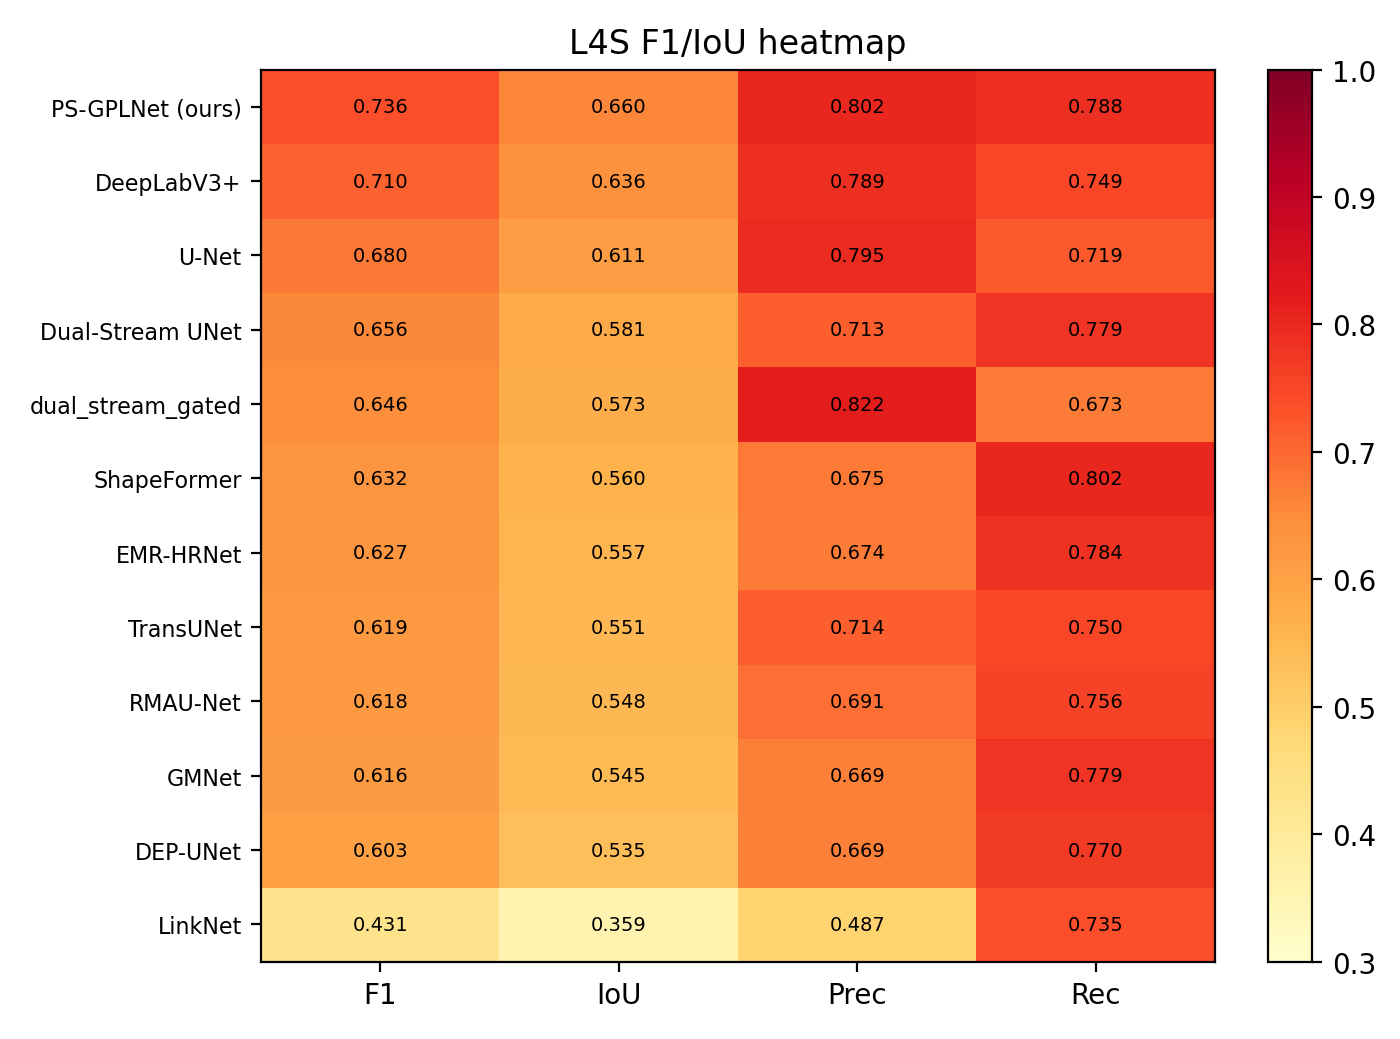
\includegraphics[width=\linewidth]{figures/fig_l4s_heatmap.png}
\caption{Landslide4Sense precision/recall/F1/IoU heatmap.}
\label{fig:l4s_heatmap}
\end{figure}

\begin{figure}[!ht]
\centering

\includegraphics[width=\linewidth]{figures/fig_bijie_heatmap.png}
\caption{Bijie precision/recall/F1/IoU heatmap.}
\label{fig:bijie_heatmap}
\end{figure}

\begin{figure}[!ht]
\centering
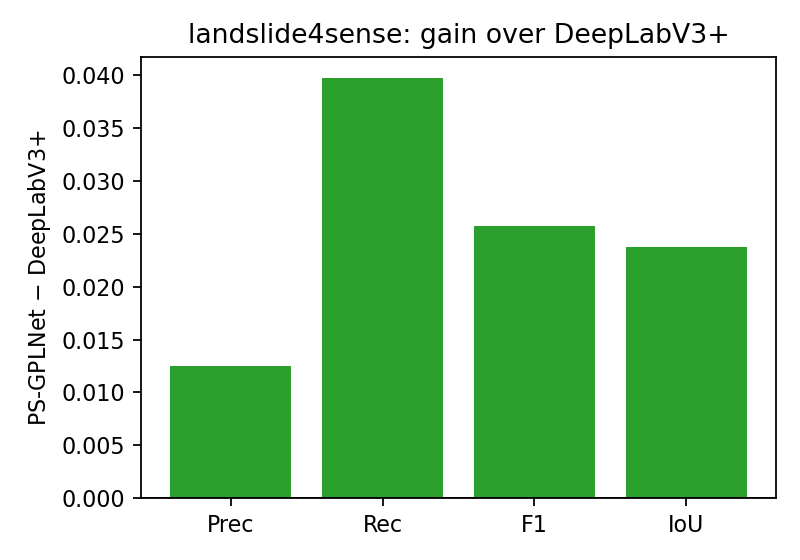
\includegraphics[width=\linewidth]{figures/fig_l4s_delta_deeplab.png}
\caption{Landslide4Sense: PS-GPLNet minus DeepLabV3+ at best epoch.}
\label{fig:l4s_delta}
\end{figure}

\begin{figure}[!ht]
\centering
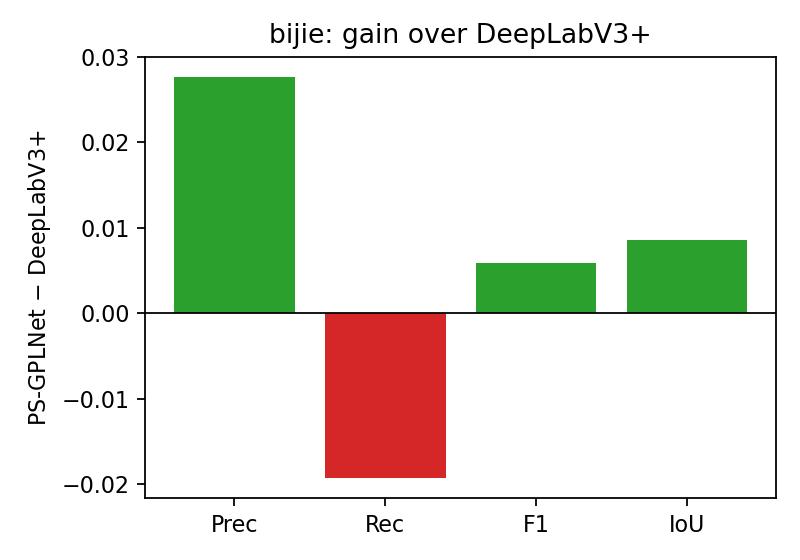
\includegraphics[width=\linewidth]{figures/fig_bijie_delta_deeplab.png}
\caption{Bijie: PS-GPLNet minus DeepLabV3+ at best epoch.}
\label{fig:bijie_delta}
\end{figure}

Training curves for PS-GPLNet are shown in Figure~\ref{fig:l4s_curves} and Figure~\ref{fig:bijie_curves}. Precision--recall operating points for all models appear in Figure~\ref{fig:l4s_pr} and Figure~\ref{fig:bijie_pr}.

\begin{figure}[!ht]
\centering
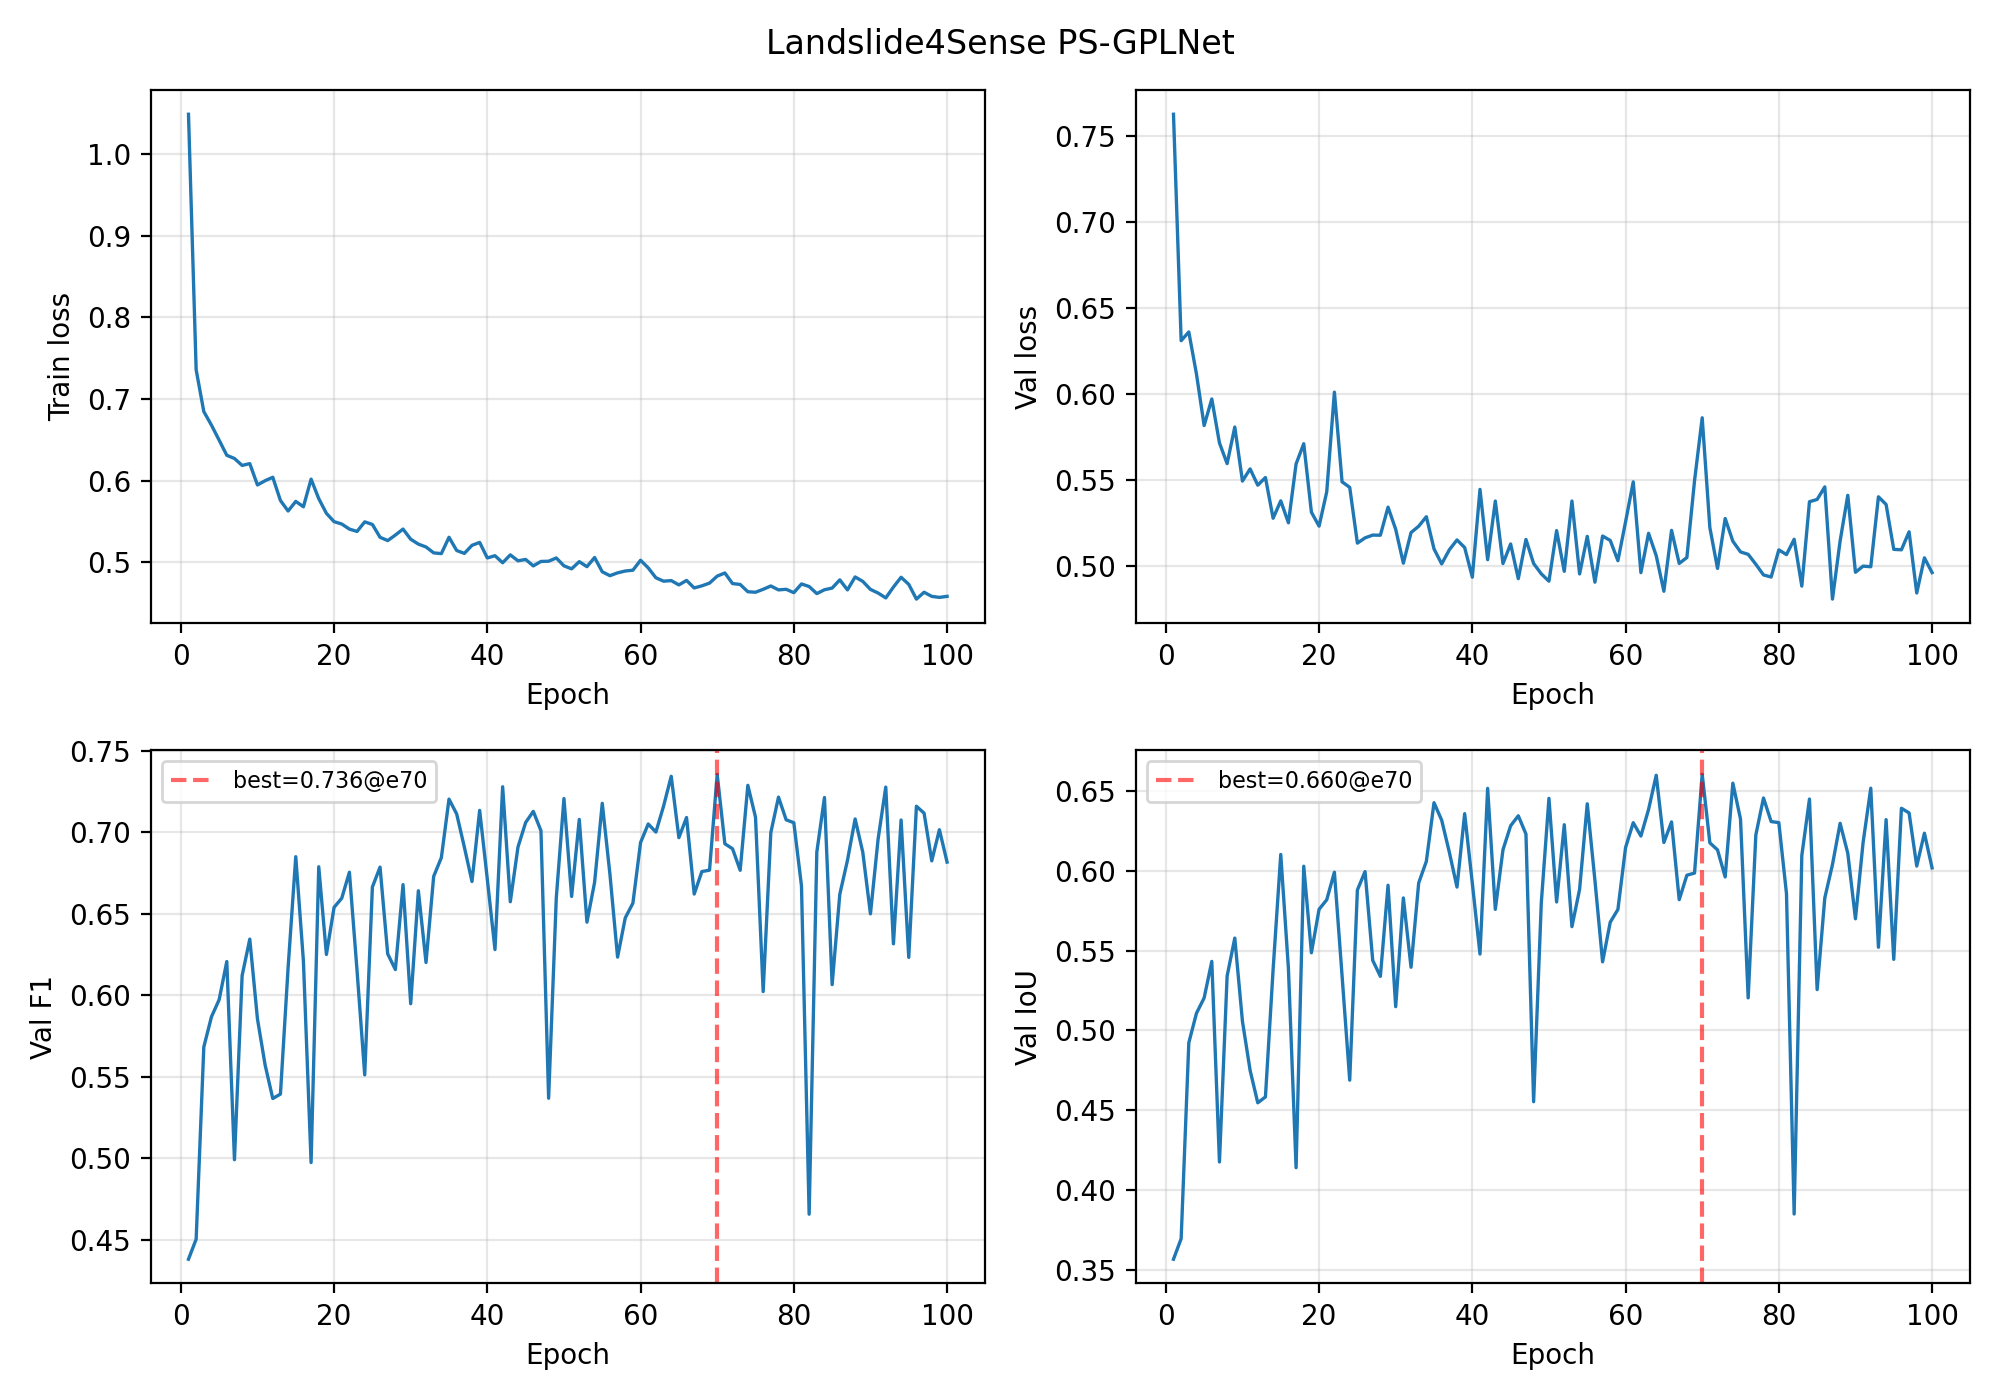
\includegraphics[width=\linewidth]{figures/fig_l4s_curves.png}
\caption{PS-GPLNet training dynamics on Landslide4Sense.}
\label{fig:l4s_curves}
\end{figure}

\begin{figure}[!ht]
\centering
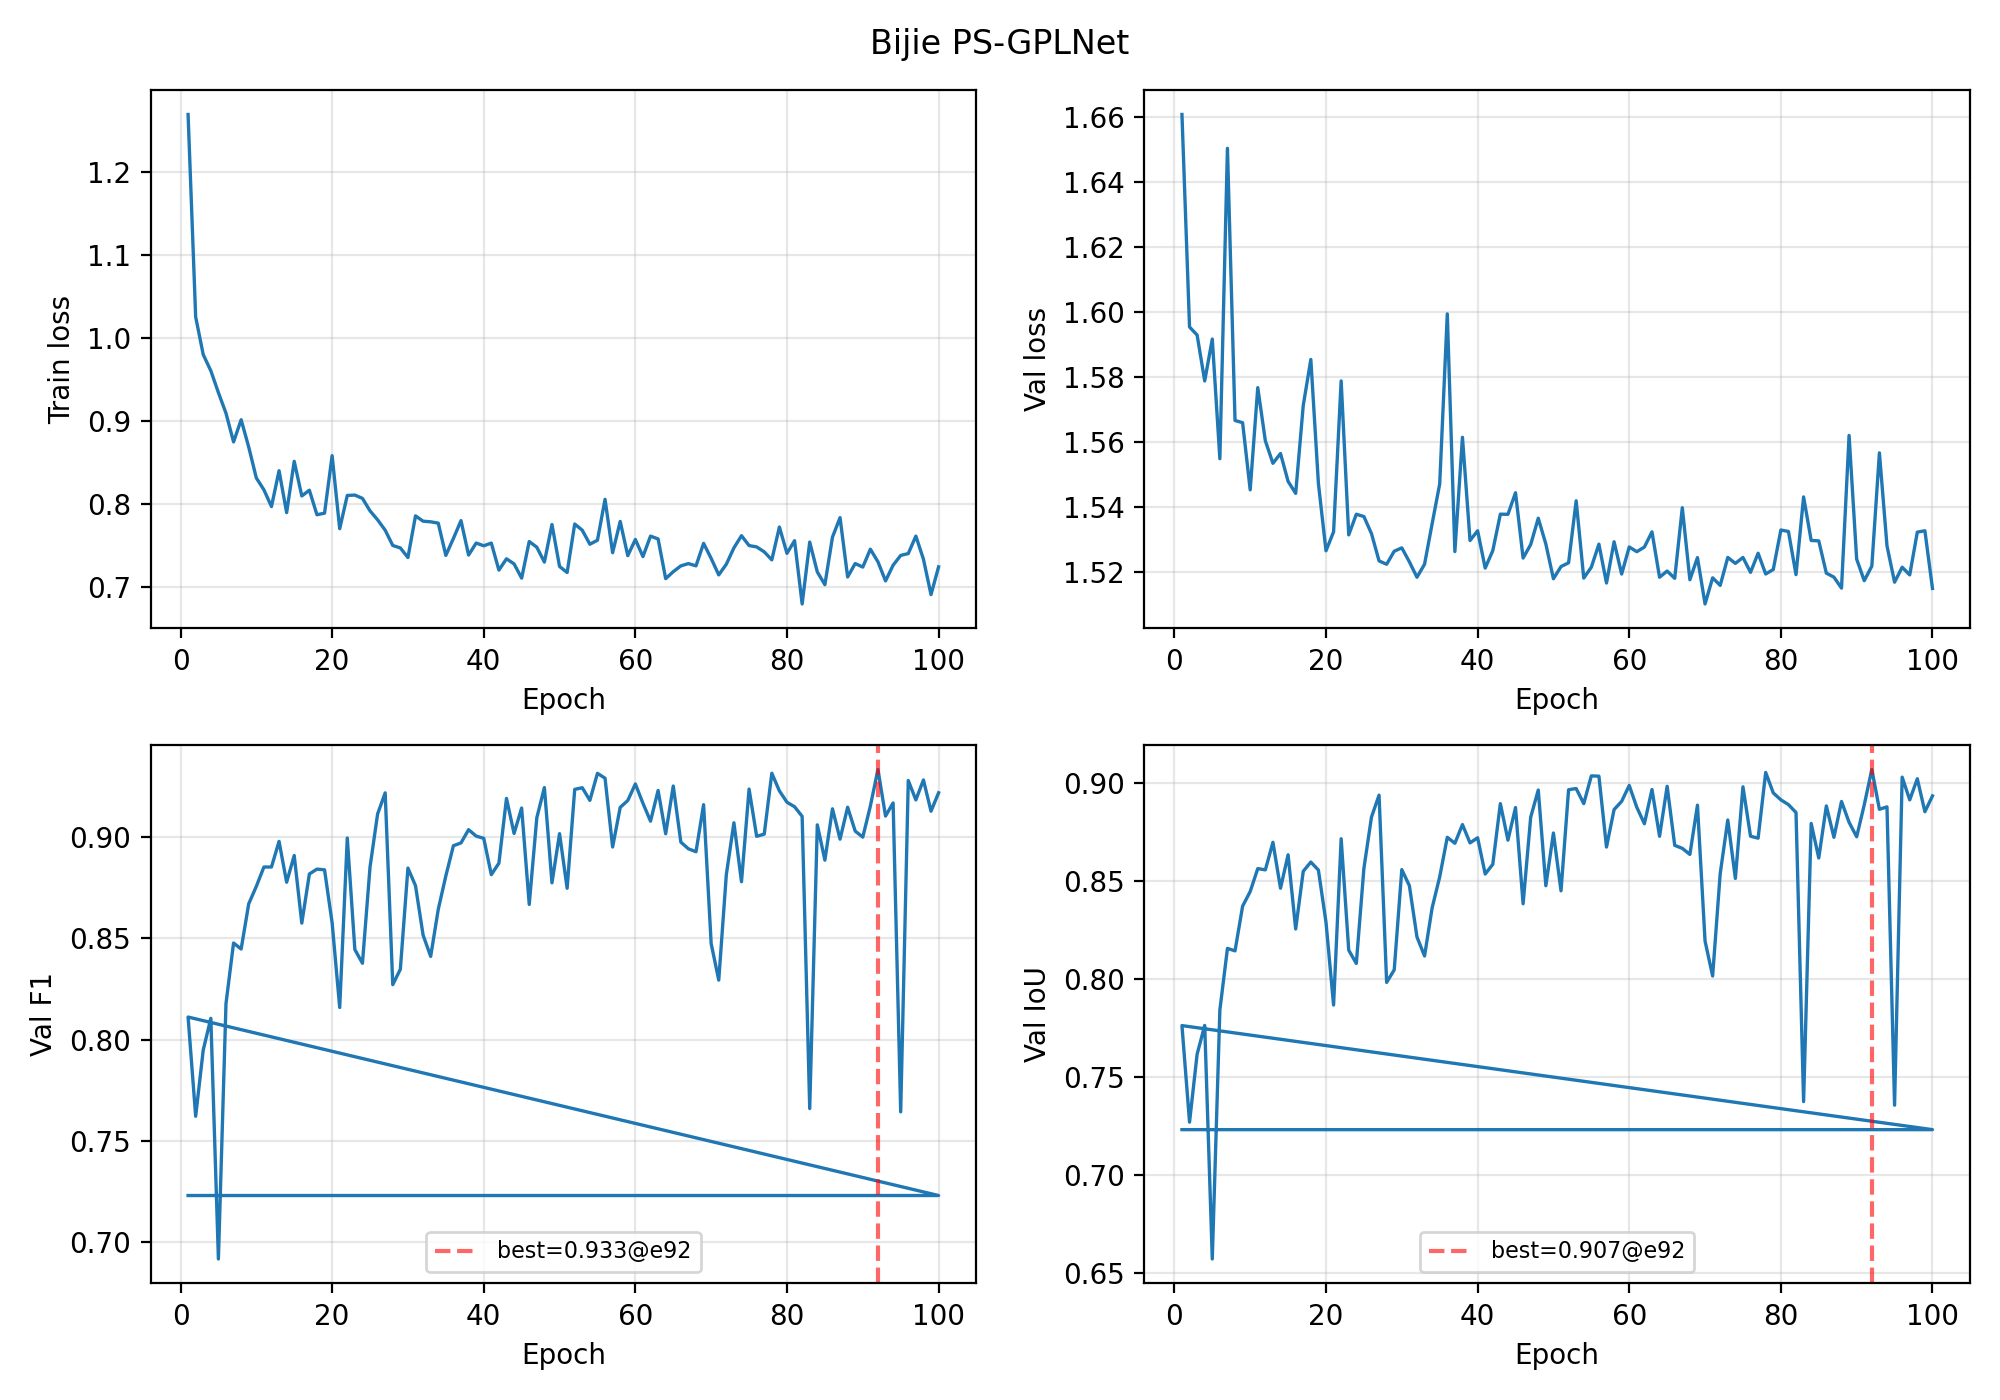
\includegraphics[width=\linewidth]{figures/fig_bijie_curves.png}
\caption{PS-GPLNet training dynamics on Bijie (best F1 at epoch 92).}
\label{fig:bijie_curves}
\end{figure}

\begin{figure}[!ht]
\centering
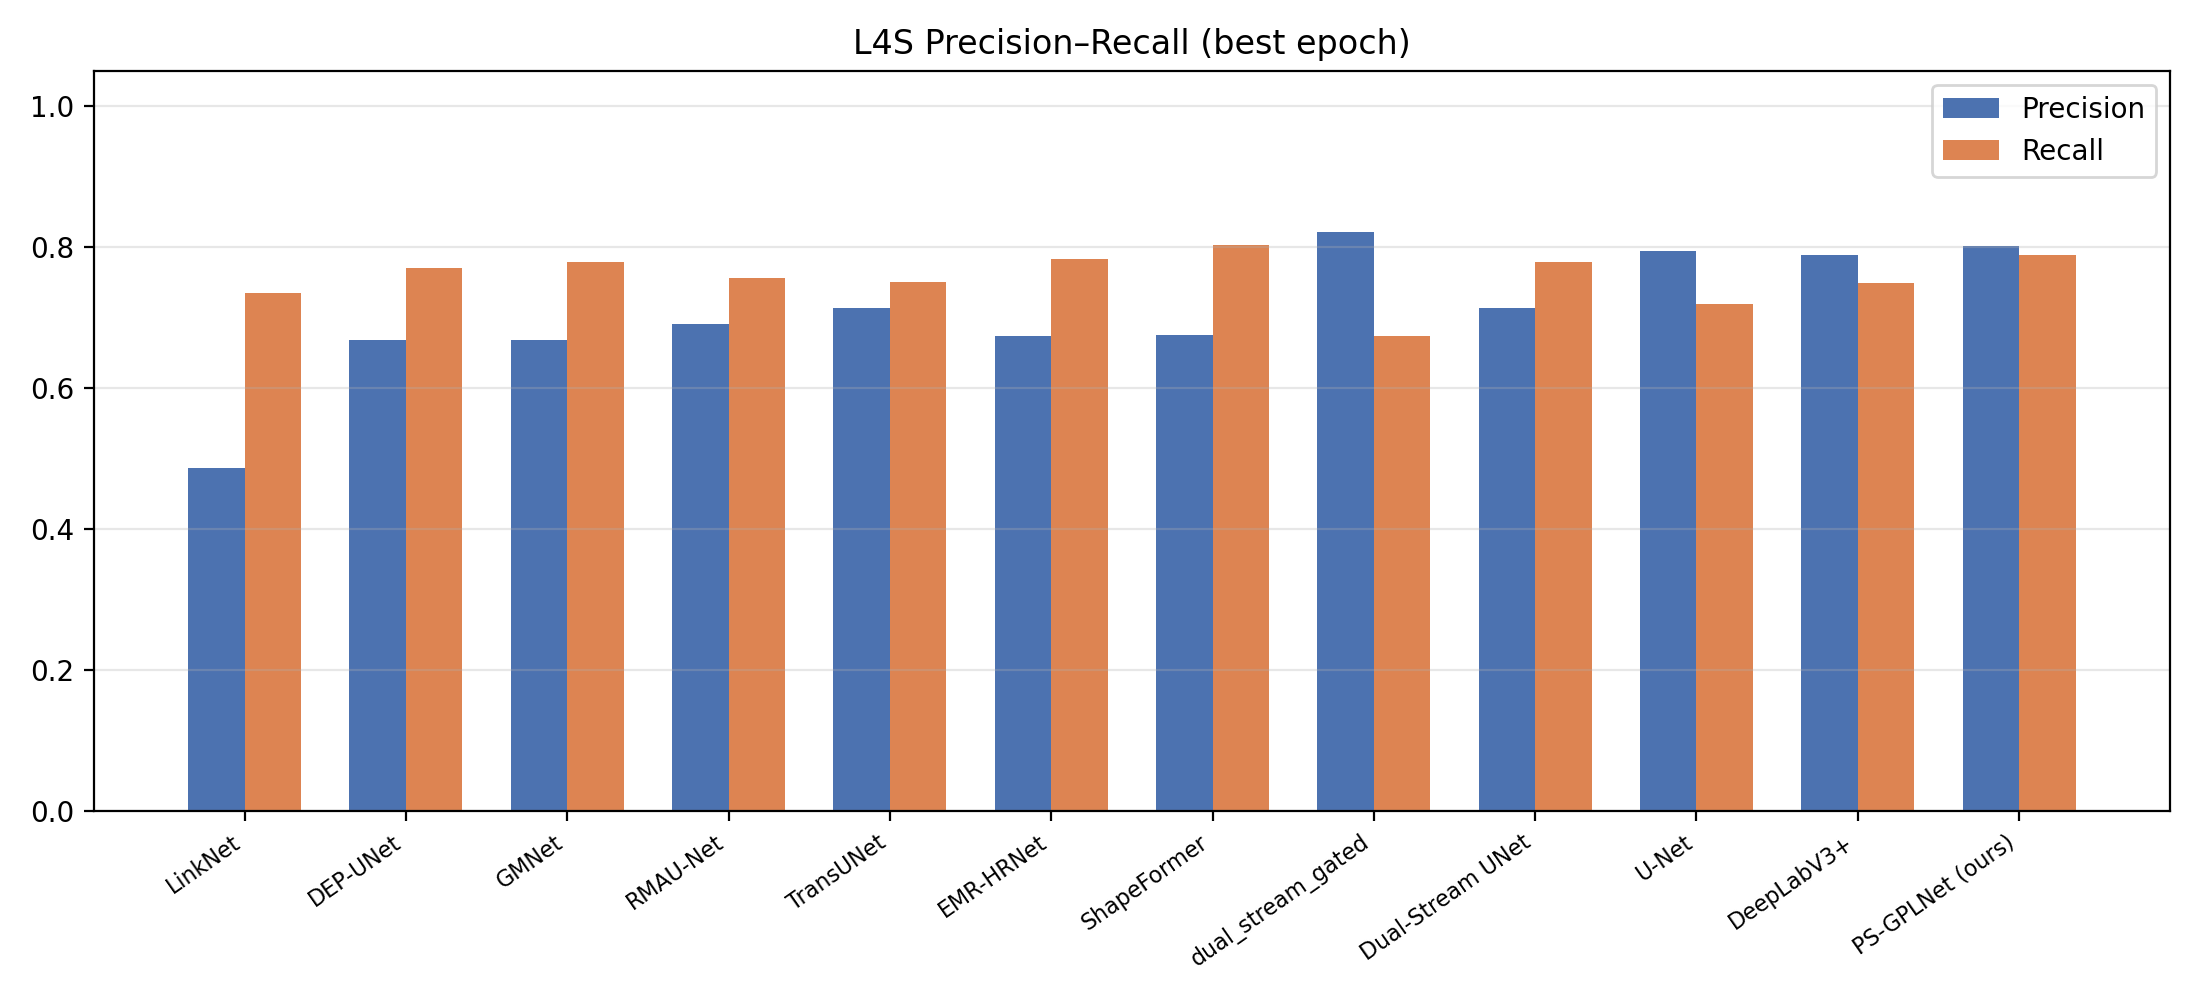
\includegraphics[width=\linewidth]{figures/fig_l4s_pr.png}
\caption{Precision--recall comparison on Landslide4Sense (best epoch per model).}
\label{fig:l4s_pr}
\end{figure}

\begin{figure}[!ht]
\centering
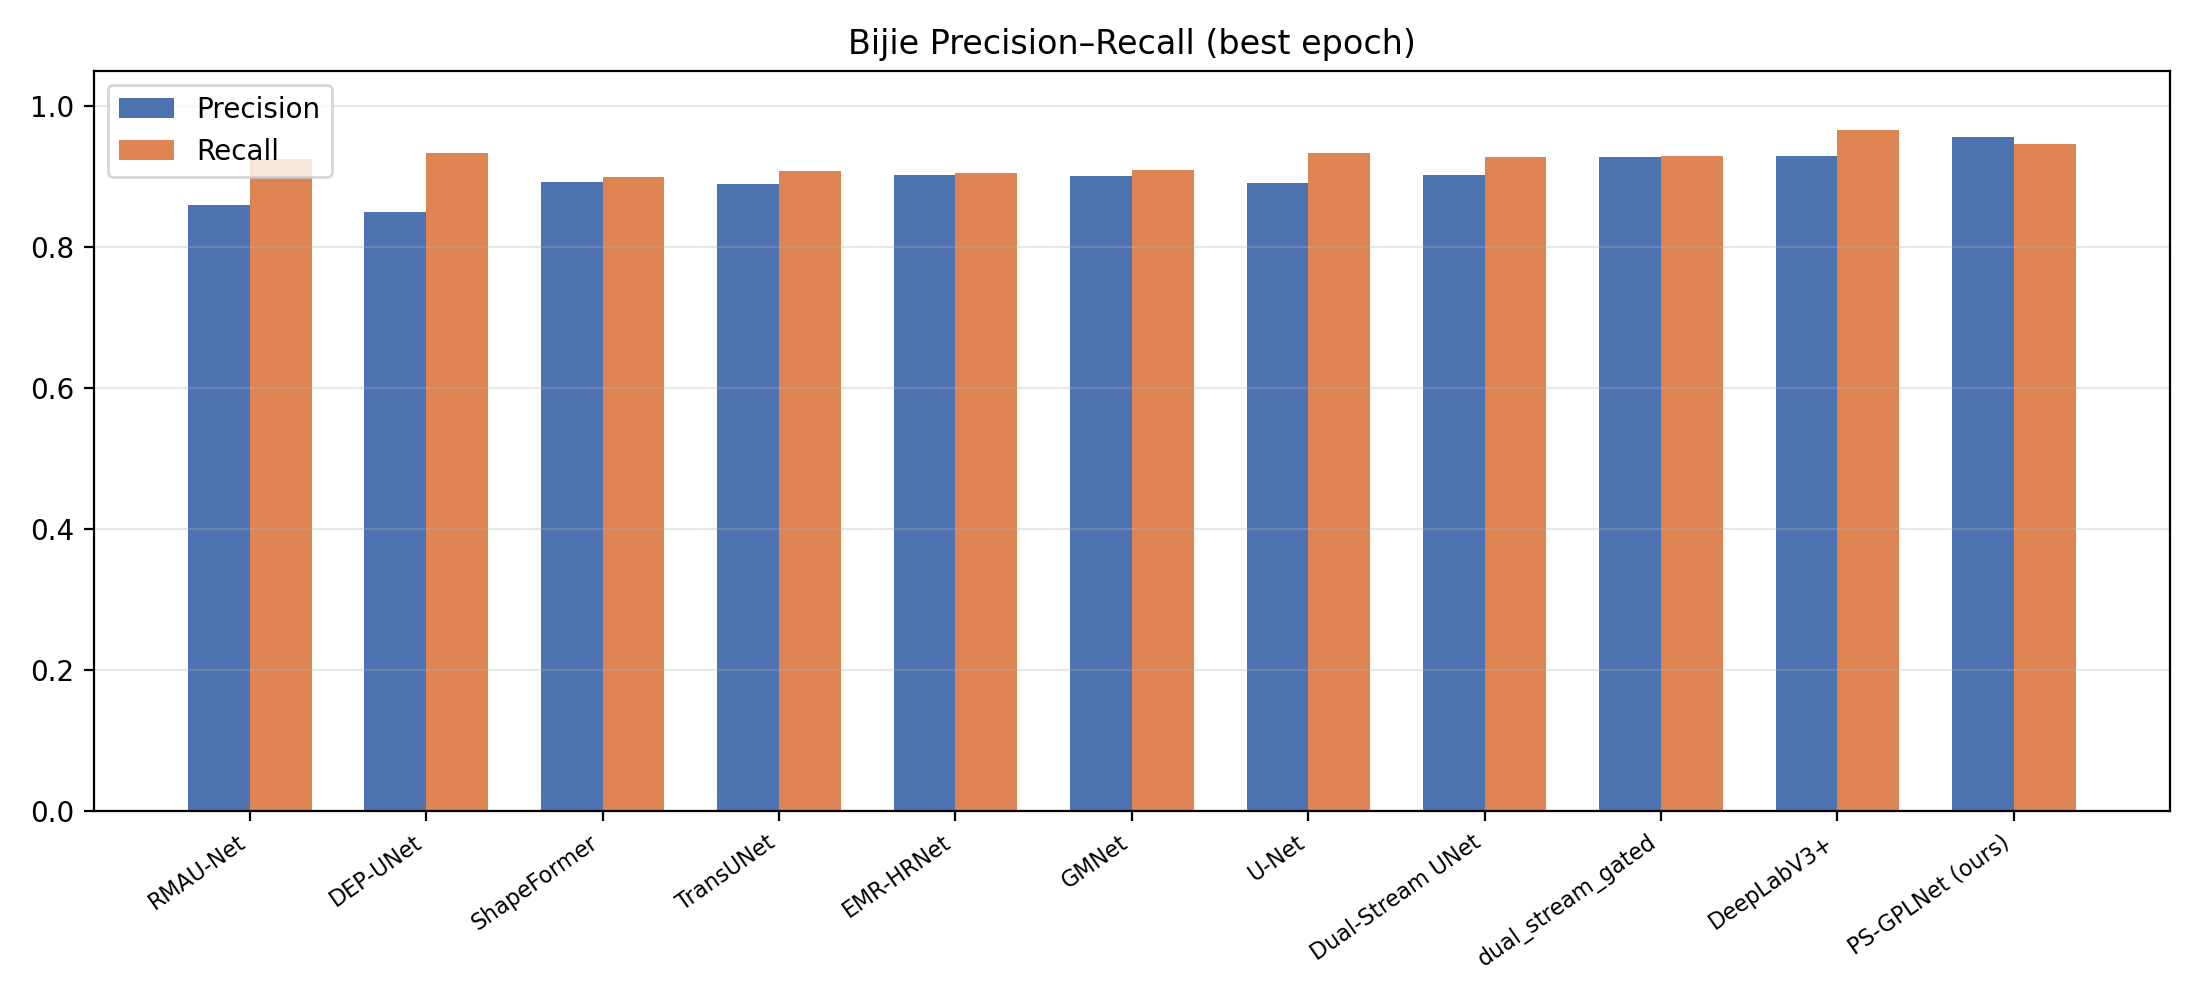
\includegraphics[width=\linewidth]{figures/fig_bijie_pr.png}
\caption{Precision--recall comparison on Bijie (best epoch per model).}
\label{fig:bijie_pr}
\end{figure}

\subsection{Qualitative results}
Representative Bijie and Landslide4Sense patches are shown in Figure~\ref{fig:bijie_qual} and Figure~\ref{fig:l4s_qual}. On Bijie, polygons are large and coherent; PS-GPLNet heatmaps concentrate on scarps and debris fans while suppressing homogeneous steep slopes. On Landslide4Sense, scars are smaller and more variable across regions; the model still recovers deposit extent but confuses some spectrally similar bare soil in shadowed valleys---consistent with the precision--recall trade-off in Table~\ref{tab:l4s}.

\onecolumn
\vspace{0.4em}
{\centering

\includegraphics[width=\textwidth]{figures/fig26_bijie_qual.png}\par
\vspace{0.35em}
\captionof{figure}{Qualitative results on Bijie validation samples: RGB, ground truth, prediction, and probability heatmap.}
\label{fig:bijie_qual}
\vspace{0.8em}

\includegraphics[width=\textwidth]{figures/fig27_l4s_qual.png}\par
\vspace{0.35em}
\captionof{figure}{Qualitative results on Landslide4Sense validation samples.}
\label{fig:l4s_qual}
\par}
\vspace{0.6em}
\twocolumn

\FloatBarrier
\section{Discussion}
\paragraph{Novelty.}
Unlike susceptibility PINNs~\cite{dahal2024pinn}, PS-GPLNet produces dense masks with foundation-model context. Unlike DiGATe~\cite{islam2024digate}, routing is failure-energy equilibrium (MPEF), and encoding is pentastream with CMB---not two EfficientNets plus scalar GateFuse.

\paragraph{Limitations.}
Full-width EfficientNet-B4 training requires sufficient GPU memory on shared HPC nodes. Compact presets reduce width and backbone size without removing dual decoders. AUROC was not logged uniformly across baseline harness runs; we report thresholded F1/IoU for consistency.

\section{Conclusion}
We presented GeoPhysicsLandslideNet, a physics-closed pentastream landslide segmenter. Closing FS logic through encoding, fusion, decoding, and MPEF yields leading Bijie F1/IoU in our unified comparison and competitive Landslide4Sense scores. Future work includes ablating individual physics blocks, multi-temporal Prithvi conditioning, and coupling dynamic rainfall forcings into the moisture proxy $m$.



{\small
\bibliographystyle{unsrt}
\bibliography{bib/refs}
}

\end{document}
